
\section{Practical limitations of lazy evaluation}
\label{intro:lazy}

The following example from \cite{gustavsson:space-improvement} demonstrates the subtlety of space usage in lazy languages:

\code{
	$\klet$	& $\ixs$	& $= [1..n]$		\\
		& $x$		& $= \ihead \ \ixs$		\\
		& $y$		& $= \ilast \ \ixs$		\\
	$\kin$	& $x + y$
}

We will use GHC as a reference point for the behavior of a real implementation. When compiled with no optimisations, the execution of this program will create a thunk for each let-binding before evaluating the addition~\cite{peyton-jones:g-machine}. If we assume that addition demands its arguments left to right, the thunk for $x$ will be forced first, resulting in the value $1$. This thunk will then be overwritten with its value, which eliminates the contained reference to $\ixs$. The evaluation of $y$ entails the construction and traversal of the list $[1..n]$ until we reach its last element. In a garbage collected implementation this can be done in constant space because $\ilast$ does not hold a reference to a list cell once it has traversed it.

However, if we change the order of arguments to addition the program consumes space proportional to the length of the list:

\code{
	$\klet$	& $\ixs$	& $= [1..n]$		\\
		& $x$		& $= \ihead \ \ixs$		\\
		& $y$		& $= \ilast \ \ixs$		\\
	$\kin$	& $y + x$
}

In this case, the evaluation of $y$ entails the construction of the entire list. The list cannot be garbage collected until the thunk for $\ihead \ xs$ has been forced, because it contains a reference to its first element. This example shows that only slight modifications to a program can result in dramatic differences in space usage.

\subsubsection{All strictness analyses are incomplete}

The run time performance of many lazy programs can be improved by exploiting the \emph{strictness} properties of functions. A function $f$ is \emph{strict} if and only if $f \ \bot \equiv \bot$~\cite{peyton-jones:implementation}. This can arise for three reasons. If $f$ inspects the value of its argument when it evaluates, then it will diverge if its argument does. If $f$ always returns its argument uninspected, then the result will be $\bot$ if the argument is. Finally, $f$ may always diverge, independent of the argument value. If none of these cases apply then function is \emph{non-strict}.

For example, the $\ichoose$ function is strict in its first argument but not the others:

\code{
	$\ichoose \ b \ x \ y = \kif \ b \ \kthen \ x \ \kelse \ y$
}

When this function is applied to its three arguments, it will always require the value of $b$. On the other hand, either $x$ or $y$ may be returned, but not both. A similar example is the $\ifirst$ function which returns just its first argument while discarding the second:

\code{
	$\ifirst \ x \ y = x$
}

As $x$ is passed through to the result, it is strict in this argument. As the function body makes no reference to $y$, it is non-strict in that one. Strictness analysis~\cite{burn:strictness, wadler:projections-strictness, sekar:fast-strictness} is used to recover the strictness properties of functions. A compiler can use this information to convert a call-by-need program into a more call-by-value version without changing its meaning. For an implementation such as GHC, this amounts to identifying the let-bound variables which are passed to strict functions, and evaluating those bindings as soon as they are encountered, instead of building thunks. 

For many lazy programs, especially those performing lots of numeric computation, evaluating strict bindings early can result in substantial performance improvements. Early evaluation saves the allocation and initialisation of thunks, as well the need to update and garbage collect them once their values are demanded.

In practice, a compiler should reduce strict bindings to weak head normal form (whnf)~\cite{peyton-jones:implementation} only. Reduction to whnf eliminates outer redexes while allowing thunks to be present deep within data structures, such as at the tail position of lists. To see why, consider our first example again:

\code{
	$\klet$	& $\ixs$	& $= [1..n]$		\\
		& $x$		& $= \ihead \ \ixs$		\\
		& $y$		& $= \ilast \ \ixs$		\\
	$\kin$	& $x + y$
}

The fact that addition and $\ihead$ are strict in their arguments implies that the $xs$, $x$, and $y$ bindings can be evaluated as soon as they are encountered. If we evaluate $[1..n]$ to whnf we construct just the outer $\iCons$ cell and the program runs in constant space. However, if we were to fully evaluate $[1..n]$ before taking its head, then the program will consume space proportional to this list.

Like all compile time analyses, strictness analysis is necessarily incomplete. This is plainly obvious from our $\ichoose$ example:

\code{
	$\ichoose \ x \ y \ z = \kif \ x \ \kthen \ y \ \kelse \ z$
}

Suppose we write an expression which uses $\ichoose$ to print one of two results:

\code{
	$\iputStr \ (\ichoose \ b \ \iexpOne \ \iexpTwo)$
}

$\iputStr$ is strict in its argument, yet the question of whether it prints $\iexpOne$ or $\iexpTwo$ can only be answered by knowing the value of $b$. In general, the value of $b$ cannot be determined at compile time. Apart from bumping up against the halting problem, this fact is obvious if we consider a situation where $b$ is derived from user input.

In a typical Haskell program, many functions are concerned with processing algebraic data. Such functions are usually written with pattern matching, or with a case-expression that examines the outer constructor of the input value. case-expressions are a generalisation of if-expressions, so we have the same problem as with the $\ichoose$ example above. In general, for a particular function call we can not know what the outer constructor of its argument will be, which defeats strictness analysis in a similar manner.


\subsubsection{Space leaks can be elegantly created with $\imapAccumL$}

In a lazy functional program, a \emph{space leak} is created when unevaluated thunks reference a large amount of data, preventing it from being reclaimed by the garbage collector. This can be counter intuitive at first glance. How can an \emph{unevaluated} expression use more space than its actual result? Consider the expression $(\irange \ 1 \ 100)$ which builds the list $[1..100]$. We would expect a thunk representing the application of $\irange$ to its arguments $1$ and $100$ to use much less space than a fully evaluated list of $100$ elements.

However, consider the case where one of the arguments is a variable instead of an integer value. A thunk which represents the application $(\irange \ 1 \ n)$ contains a reference to the object $n$, and as long as the thunk is live this object cannot be garbage collected. Suppose $n$ is also a thunk, and that it references a large amount of data. While our original list remains unevaluated, this data remains live. It may be that the program's performance would be improved by forcing the list to be fully evaluated as soon as possible. This would allow the garbage collector to reclaim space used by thunks and objects that are no longer referenced. Of course, whether this would work in practice is very application specific. Factors to consider include the size of the resulting list versus the size of the retained data, whether the entire list value will actually be used by the program, whether the live data is also held live by other expressions, cache and main memory sizes, and so on.

Space leaks are especially common in lazy programs which are based around state and state transformers. For these programs, execution is divided into a sequence of steps, with a well-defined state before and after each step. The function $f$ takes the old state, some input $x$ and produces the next state and some output $y$:

\begin{center}
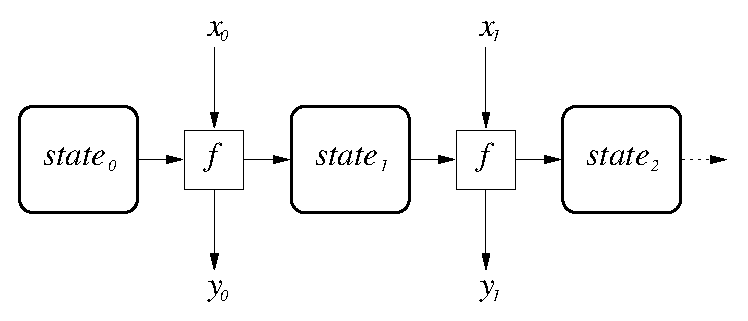
\includegraphics[scale=0.8]{1-Introduction/fig/lazy/space-leak}
\end{center}

\clearpage{}
In Haskell, this pattern of computation is expressed by the function $\imapAccumL$ which has type:
$$\imapAccumL :: (\istate \to x \to (\istate, y)) \to \istate \to [x] \to (\istate, [y])$$

$\imapAccumL$ takes a transition function, an initial state, a list of inputs and produces the final state and the list of outputs. Many programs use a similar pattern of computation, though not all express it with $\imapAccumL$. Consider an interactive program such as a computer game. We could imagine that $\istate$ is a description of the game world, $x$ is the user input, $y$ is a description of the user display, and $f$ is the game logic which computes a new state and display based on the input.

For a computer game, the state could consist of the player's position, surrounding terrain, current enemy positions, remaining ammunition, and so on. A space leak is created when the program fails to demand the entire $y$ value after each step. Suppose that $y$ includes the player's score at each step of the game, but this information is not displayed in real time. Although the score at each step might be expressed by a single integer, as it depends on the current game state at least past of this structure must be kept live until the integer is fully evaluated. If a user plays the game for an hour, with a new state generated 30 times a second, then this can equate to a substantial amount of retained data. Additionally, when the score is a non-trivial function of the current state, reasoning about the \emph{amount} of space wasted becomes intractable.

In Haskell, the only practical way to deal with a complex leak is to write so called $\ideepseq$ functions that manually traverse over an entire structure to ensure it is fully evaluated. Other techniques can help, such as having the garbage collector perform leak avoiding projections~\cite{wadler:fixing-space-leaks}, but to fully cure leaks the programmer must ensure that all structures which \emph{should} be evaluated actually are. Most $\ideepseq$ functions are written to eliminate all redexes in a structure, and are therefore equivalent to the \emph{reduce to normal form} strategy from \cite{trinder:algorithm}. A built-in $\ideepseq$ function was proposed for Haskell', the successor standard to Haskell 98~\cite{haskell-prime:deepseq}, but as of November 2008 it has not been implemented in GHC. 

It is also possible to add strictness annotations to user defined data types. These annotations prevent thunks being created at certain positions in the structure, but cannot be easily be added to library defined types such as $\iMap$ and $\iList$.


\subsubsection{Case study of a space leak}

A state based space leak was encountered while the author was developing a graph coloring register allocator~\cite{chaitin:graph-coloring, smith:graph-coloring} for GHC 6.7. The algorithm is based around a graph where each node represents a program variable. An edge between two nodes represents a constraint that those two variables can not be assigned to the same register. The goal is to assign registers, visualised as colors, to each of the nodes in a way that satisfies the constraints, whilst using only the available set of registers. The algorithm proceeds by extracting a constraint graph from the code undergoing register allocation, and then attempting to color it. If this is not possible with the available colors (registers) then the algorithm modifies the code to store some variables on the stack instead of registers, and tries again. For non-pathological programs this process should converge within three or four iterations.

Graph coloring register allocation is a state based algorithm. The state consists of the current version of the code undergoing allocation, along with the constraint graph. As opposed to the $\imapAccumL$ function, there is no extra per-step input to the state transition function corresponding to the $x$ values in the previous diagram. The output $y$ values correspond to graph profiling information, such as the number of colored versus uncolored nodes remaining after each step.

When the allocator was being developed we were well aware of space leaks and their causes. The intended operation of the algorithm was to build a complete constraint graph, attempt to color it, and if that failed to build a new graph and leave the old one for the garbage collector. We knew that if the program retained any references to the profiling information for old graphs, then this would prevent those graphs from being garbage collected. If this happened we would have a space leak, so we made considerable effort \emph{not} to retain profiling information unless it was explicitly requested. We reasoned that if the user requested profiling information then they would not mind if the allocator ran a little slower due to retained data, as this was not a common operation.

 However, once it was written, an examination of heap space~\cite{sansom:profiling} used by the allocator revealed the following:

\begin{center}
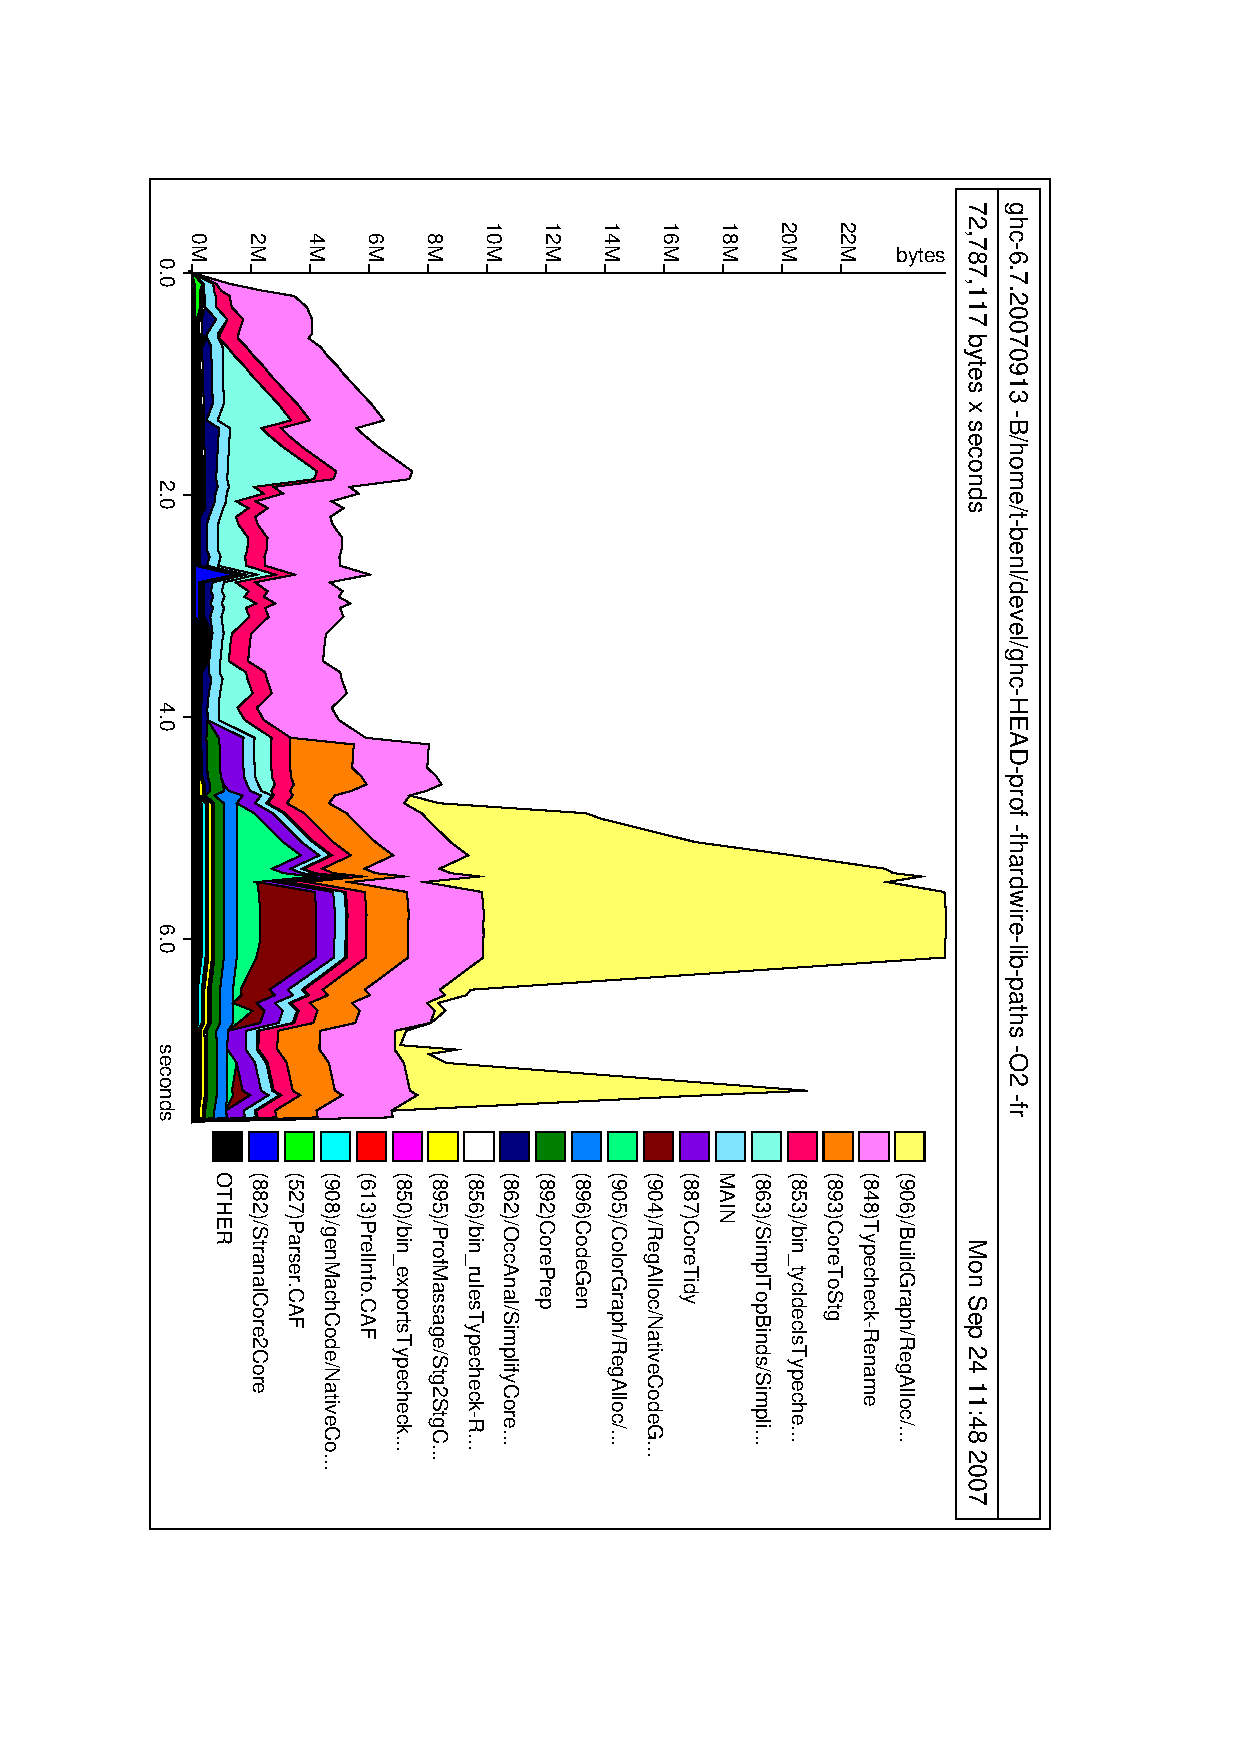
\includegraphics[scale=0.5, angle=90]{1-Introduction/fig/lazy/ghc-sha1-leak.epsi}
\end{center}

The two large spikes in space usage that appear around 6 and 7 seven seconds are directly attributable to the register allocator. This is when performing allocation for the \texttt{SHA1.hs} module from the darcs 1.0.8 source code. Object type profiling revealed that most of the space was taken up by thunks representing function applications.

As to the exact cause of the leak, we are not sure. We could imagine that when the compiler emits a particular compiled machine instruction, this action demands the result of register allocation for that instruction. The registers allocated to a particular instruction depend on what other registers are assigned to surrounding instructions. We could then imagine a section of graph in the final state of the allocator being demanded. This in turn might demand larger sections of graph from previous states, along with parts of the various intermediate versions of assembly code that we tried to find allocation solutions for. 

Good research has been done on formally analysing the space usage of call-by-need programs~\cite{gustavsson:space-improvement, bakewell:space-usage}. However, trying to reason about the exact space behavior of a three thousand line program, compiled with a production compiler that incorporates tens, if not hundreds of individual optimisations is another matter entirely. We plainly admit that our reasoning is little but inspired guess work.

What we do know is that using a $\ideepseq$ function to force the graph to be fully constructed before coloring cured the worst of the problem. This result was obtained through experimentation and frequent consultation with the heap usage profile. The following profile is for the final version:

\begin{center}
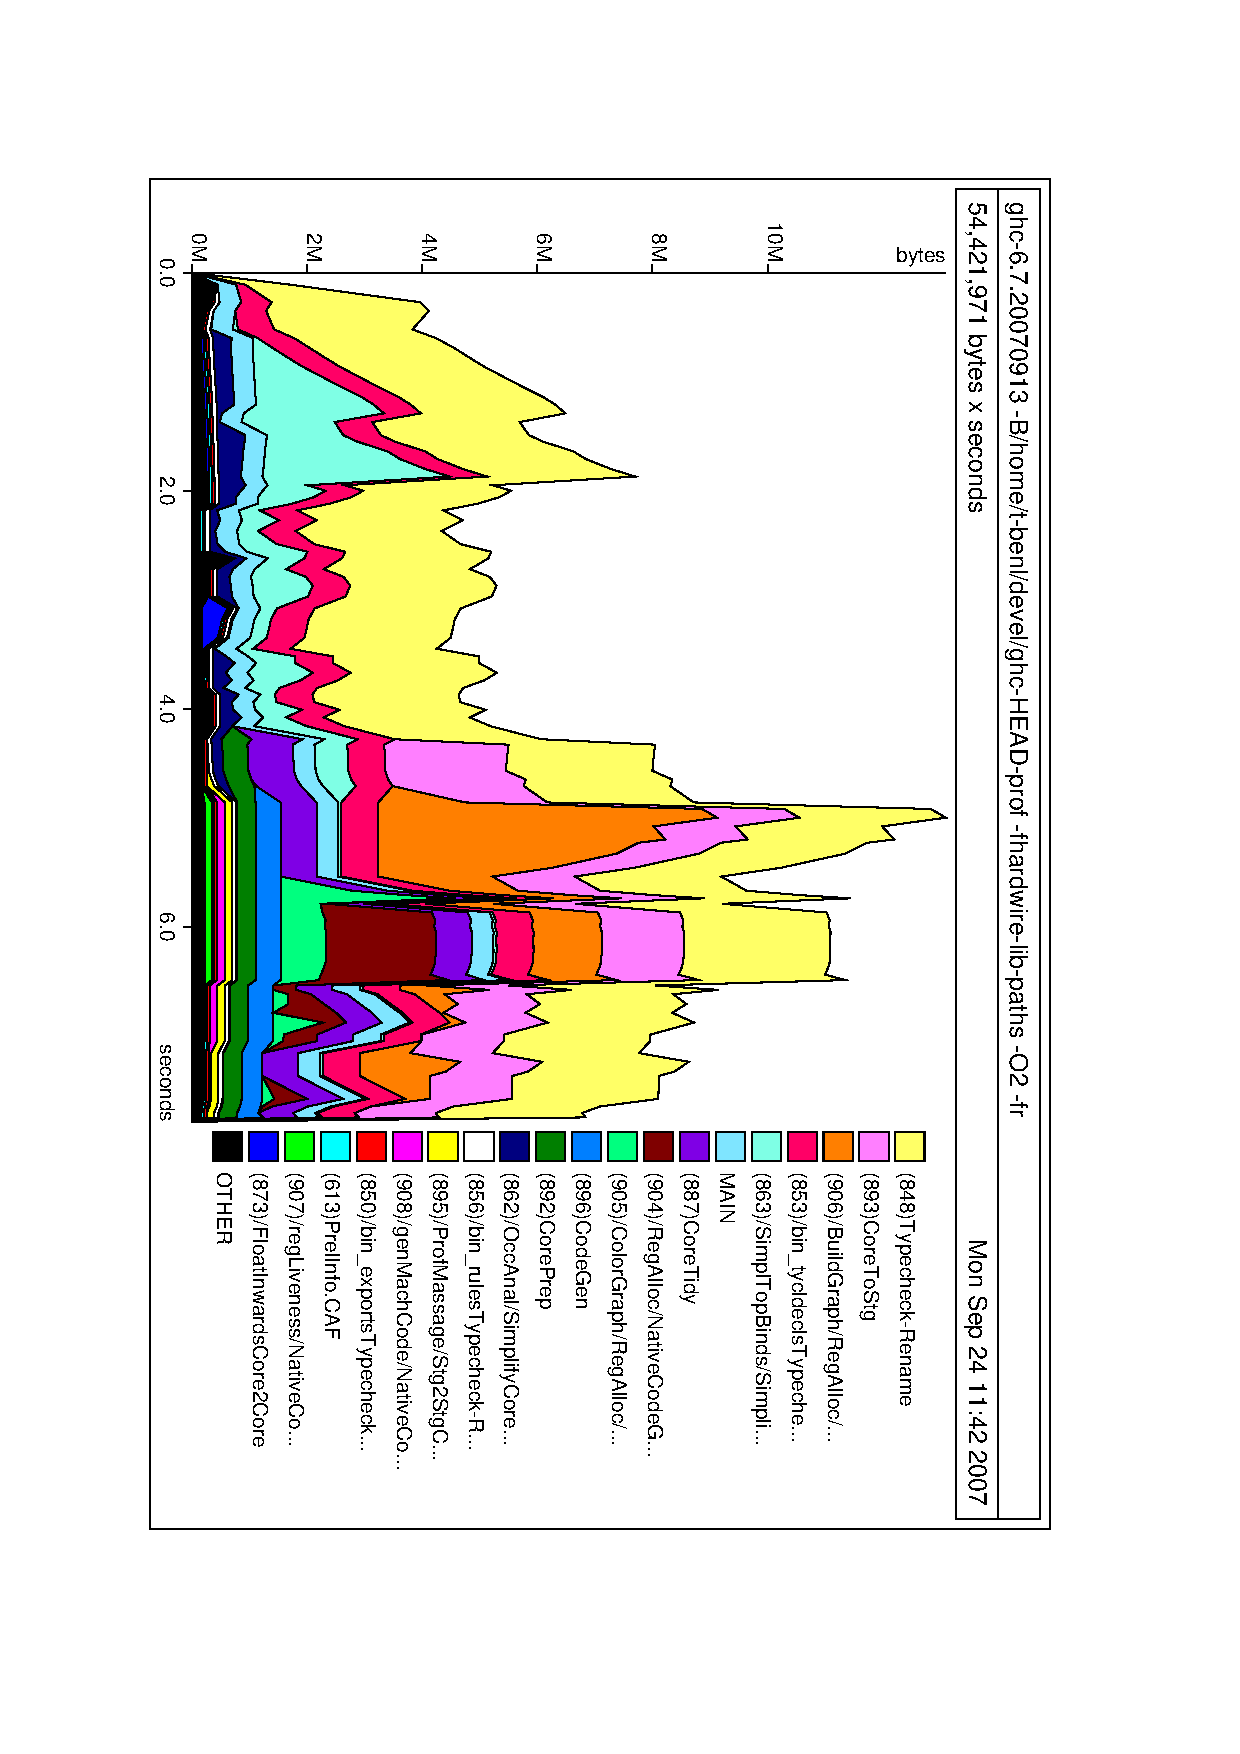
\includegraphics[scale=0.5, angle=90]{1-Introduction/fig/lazy/ghc-sha1-ok.epsi}
\end{center}

In this version the large spikes in space usage have been reduced, resulting in a peak usage around half of the unforced version. We conjecture that the remaining cost attributed to \texttt{(906)/BuildGraph/RegAlloc} is mostly due to the legitimate construction of the graph during allocation, though once again we can not be sure. We deemed the profile acceptable, and moved on to other things.

We glean several points from this experience. Firstly, although a programmer may write what they feel is a state based program, if it is expressed in a lazy language then it may not behave that way at runtime. Secondly, the exact cause of space leaks in large lazy programs can be very hard to reason about. That being said, although the \emph{problem} may be hard to characterise, the solution is well understood. Forcing thunks to values eliminates their contained references and frees up objects for the garbage collector. 

On a philosophical note, we feel there is an immense practical difference between optimisation and control. Having a large number of optimisations in a compiler is all well and good, but if the compiled code \emph{still} doesn't run fast enough then the language (and/or compiler) must provide enough additional control for the programmer to step in and fix the problem. If this is not possible then the programmer will be forced to use a different language, and if that happens more than once then they will be unlikely to choose the same system for their next project.

In this case we were able to fix the problem. However, we do note the irony of writing extra code to manually force the evaluation of expressions that we did not intend to be suspended in the first place. We cannot, off hand, think of a single place in the register allocator code where lazy evaluation was used for a useful purpose. 

We are not suggesting that laziness is never useful, more that it depends on the application. For a selection of programs from the nofib benchmark suite~\cite{partain:nofib}, Harris~\cite{harris:feedback-parallelism} gives the percentage of allocated thunks that were actually evaluated at run-time. In the 20 programs considered, 9 ended up evaluating at least 99\% of their thunks, 14 evaluated at least 90\%, while only one evaluated less than 80\%. 

The fact that a program evaluates almost all of its thunks does not imply it does not make use of laziness. For example, if we use laziness to evaluate the expression $\isum \ [0..100]$ in constant space, then all the thunks in the list will be forced. The application of $\isum$ to a $\iCons$ cell demands the element value as well as the tail of the cell. However, the fact that a program evaluates 99\% of its thunks would suggest that it is not creating lazy lists where the spine is evaluated but the majority of the elements are not. It would also suggest that the program is not using the ``sexier'' lazy structures, such as infinite game trees \cite{hughes:fp-matters}. 




